\chapter{Analiza ruchu sieciowego}
	\label{chap:analiza}
	\section{Narzędzie Netfilter}
		Jako systemu analizującego ruch sieciowy wykorzystam pakiet Netfilter konfigurowany za pomocą iptables.
	\section{Ogólny zarys}
		Netfilter jest oprogramowaniem pozwalającym na filtrowanie pakietów, ich translacje (NAT) oraz inne manipulację.
		Od wersji jądra 2.4.x, pakiet netfilter jest umieszczony wewnątrz niego.
		Potrafi on dopasowywać analizowane pakiety ze względu na szeroką gamę kryteriów, jak również przeprowadzić szereg operacji na danych pakietach.
	\section{Zasada działania}
		Netfilter posiada 4 zdefiniowane tablice: raw, mangle, nat, filter, oraz 5 łańcuchów: PREROUTING, INPUT, FORWARD, OUTPUT, POSTROUTING.
		Kolejność przechodzenia pakietu przez tabele i łańcuchy obrazuje rys. \ref{fig:flowchart}.\\
		\begin{figure}[h]
			\centering
				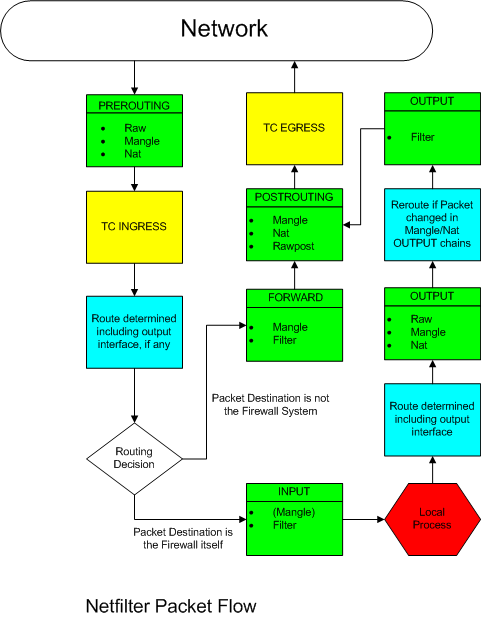
\includegraphics[width=280px]{Netfilter.png}
				\caption{Przepływ pakietów w netfilter, źrodło \cite{netfilter}}
				%http://www.shorewall.net/images/Netfilter.png
				\label{fig:flowchart}
		\end{figure}
		Gdy pakiet dochodzi do komputera na którym jest netfilter, zostaje on przekazany do łańcucha PREROUTING. Następnie, następuje decyzja o routowaniu pakietu, i w zależności czy pakiet jest kierowany do lokalnego komputera, jest kierowany do łańcucha INPUT, bądź w przypadku gdy ma zostać przekazany dalej, do łańcucha FORWARD oraz POSTROUTING.\\
		W przypadku, gdy pakiet jest generowany przez nasz komputer, zostaje on przejęty przez łańcuch OUTPUT, a następnie POSTROUTING.

		Pierwszą tablicą przez którą przechodzi pakiet, jest tablica \textit{raw}. W tym miejscu możemy oznaczyć pakiet targetem TRACE, który spowoduje logowanie każdej reguły do której pakiet będzie pasował. Wykorzystywane jest to przy debugowaniu sieci bądź firewalla.
		Inna opcją która może pojawić się jedynie w tablicy raw, jest target NOTRACK. Spowoduje on nieoznaczenie pakietu przez moduł \textit{conntrack}, który rejestruje pakiety i rozpoznaje je jako istniejące połączenia.

		Następna tablicą do której zostaje przekazany pakiet, jest tablica \textit{mangle}.
		W tablicy tej możemy manipulować wartościami TTL.

		Kolejną tablicą przetwarzającą pakiet, jest tablica \textit{nat}.
		W tablicy tej możemy manipulować adresami pakietowymi.
		W zależności, czy naszym celem jest SNAT cz DNAT, używamy do tego odpowiednich łańcuchów PREROUTING i POSTROUTING

		Ostatnią tablicą, która przetwarza pakiety, jest tablica \textit{filter}. Jest to tablica w której powinno się umieszczać wszystkie reguły dotyczące filtrowania pakietów. 
		Jeżeli nie zostanie jawnie podana tablica, domyślną tablicą jest tablica \textit{filter}.

		Jeżeli pakiet zostanie przetworzony przez całą ścieżkę w firewallu i nie zostanie podjęta decyzja o zaakceptowaniu bądź odrzuceniu pakietu, zostaje zastosowana polityka odpowiedniego dla tego pakietu łańcucha głównego, tj. INPUT, OUTPUT, FORWARD.
		Politykami mogą być TARGET-y terminujące, tj. ACCEPT, REJECT, DROP.
	\section{Najważniejsze kryteria dopasowania}
		Netfilter posiada bogaty wachlarz możliwości dopasowywania pakietów
		\begin{description}
			\item[-{}-source, -{}-src, -s \param{adres} ] \hfill \\
				dopasowuje adres źródłowy pakietu do podanego jako \textit{adres}
			\item[-{}-destination, -{}-dst, -d \param{adres}] \hfill\\
				dopasowuje adres docelowy pakietu do podanego jako \textit{adres}
			\item[-{}-protocol, -p \textit{\textless protocol \textgreater}] \hfill \\
				dopasowuje protokół używany przez pakiet.\\
				Najczęściej używane protokołu to: \textit{tcp},\textit{udp},\textit{icmp}
			\item[-{}-source-port, -{}-sport \textit{\textless port \textgreater} ]\hfill\\
				dopasowuje port źródłowy pakietu.\\
				Aby użyć tego dopasowania należy zdefiniować protokół.
			\item[-{}-destination-port, -{}-dport \textit{\textless port \textgreater}] \hfill \\
				dopasowuje port docelowy pakietu.\\
				Aby użyć tego dopasowania należy zdefiniować protokół.
			\item[-{}-tcp-flags \textit{\textless maska \textgreater \textless flagi \textgreater}] \hfill \\
				dopasowuje pakiet, jeżeli wszystkie \textit{flagi} są ustawione oraz wszystkie flagi niewymienione w \textit{flagi} a uwzględnione w \textit{maska} są nieustawione
			\item[-{}-mac-source \textit{\textless mac-adres \textgreater}] \hfill \\
				dopasowuje pakiet na podstawie źródłowego adresu sieciowego. Adres podawany jest w formacie: AA:BB:CC:DD:EE:FF.
			\item[-{}-in-interface, -i \param{interface}] \hfill \\
				dopasowuje pakiet ze względu na interface sieciowy na którym dany pakiet się pojawił	
			\item[-{}-out-interface, -o \param{interface}] \hfill \\
				dopasowuje pakiet ze względu na interface sieciowy przez który pakiet będzie wysyłany
			\item[-{}-limit \param{ilość}/\param{czas}] \hfill \\
				dopasowuje pakiety, jeśli ich ilość nie przekracza \textit{ilość} w okresie \textit{czas}.\\
				\textit{Czas} może przyjmować wartości: second, minute, hour, day.
		\end{description}
	\section{Najważniejsze działania}
		Jeżeli pakiet zostanie dopasowany, netfilter może wykonać jedną ze zdefiniowanych akcji a pakiecie. W przypadku niezdefiniowania akcji, pakiet przechodzi do kolejnych reguł w firewallu a w firewallu zostaje zwiększony licznik dopasowanych pakietów dla danej reguły.\\
		Dopasowany pakiet zostaje wysłany do wybranego targetu poprzez opcję -j, np: -j~ACCEPT.
		\begin{description}
			\item[ACCEPT] \hfill \\
				dany pakiet zostaje zaakceptowany i nie przechodzi przez dalszą filtrację
			\item[REJECT] \hfill \\
				odrzucenie pakietu z wysłaniem informacji do adresata. Domyślna wartość odpowiedzi to icmp-port-unreachable.\\
				Istnieje możliwość ustawienia odpowiedzi wysyłanej do adresata poprzez atrybut -{}-reject-with \param{type},
				gdzie \textit{type} jest jednym z zdefiniowanych komunikatów:
				\begin{itemize}
					\item icmp-net-unreachable
					\item icmp-host-unreachable
					\item icmp-port-unreachable
					\item icmp-prot-unreachable
					\item icmp-net-prohibited
					\item icmp-host-prohibited
					\item icmp-admin-prohibited.
				\end{itemize}
			\item[DROP] \hfill \\
				odrzucenie pakietu, bez wysyłani informacji zwrotnej do adresata. Pakiet zostaje "upuszczony".
			\item[LOG] \hfill \\
				pakiet zostaje wysłany do systemu logowania jądra. Jest to nieterminatorowy target, to znaczy, że po dopasowaniu pakietu, zostaje on zalogowany, a następnie przechodzi przez dalszą część firewalla.\\
				Najczęściej jest on stosowany wraz z opcją -{}-log-prefix, który dodaje prefix w systemie logowania. Pozwala on na późniejsze odróżnienie poszczególnych logów od siebie.
			\item[TTL] \hfill \\
				pozwala na manipulację wartościami TTL. Zalecane jest niezmienianie tej wartości, jednak w praktyce, są sytuacje w których zmiana wartości TTL jest potrzebna.\\
				Możliwe opcje przekazywane do tego targetu:
				\begin{description}
					\item[-{}-ttl-set \param{wartość}] \hfill \\
						ustawia wartość ttl na podaną
					\item[-{}-ttl-inc \param{wartość}] \hfill \\
						zwiększa wartość ttl o podaną wartość
					\item[-{}-ttl-dec \param{wartość}] \hfill \\
						zmniejsza wartość ttl o podaną wartość
				\end{description}
			\item[REDIRECT] \hfill \\
				target ten przekierowuje pakiet na siebie. Istnieje również możliwość możliwość zmiany portu w danym pakiecie poprzez opcję: -{}-to-ports \param{port}.
				Aby użyć opcji -{}-to-ports, należy określić protokół -p \param{protokół}
			\item[SNAT] \hfill \\
				pozwala zmienić adres źródłowy dopasowanego pakietu. Określenie nowego adresu źródłowego dokonujemy za pomocą opji:\\
				-{}-to-source \param{adres} [:\textit{port}[\textit{-port}]]\\
				gdzie \textit{port} jest opcjonalnym parametrem określającym port, bądź zakres portów. Aby zdefiniować port(y) należy zdefiniować protokół.
			\item[DNAT] \hfill \\
				pozwala zmienić adres docelowy oraz port dopasowanego pakietu. Określenie nowego adresu docelowego dokonujemy za pomocą opji:\\
				-{}-to-source \param{adres} [:\textit{port}]\\
				Aby móc zdefiniować port, należy określić protokół.
		\end{description}

